The acceptance tests performed are based on the documentation provided by the team. \\

\subsection{Acceptance tests based on use cases}
The tests were developed taking the use cases described in the RASD and modifying them according to what was finally implemented as explained in the ITD. \\
The “expected steps” describe the flow we would expect to follow to complete a test, before coming into contact with the finished prototype. While the “real steps” are the steps followed to complete the use case when using the prototype. \\

\begin{table}[H]
    \centering
    \begin{tabular}{p{3cm}p{10cm}}
    \textbf{Test ID} & AT-001-SIGN\_UP \\ \hline
    \textbf{Based on} & Registration as a Normal User to SafeStreets \\ \hline
    \textbf{Pre-requisites} & - \\ \hline
    \textbf{Expected steps} & 
        \begin{enumerate} \itemsep0em
            \item The System shows the registration page.
            \item Input the following data: email, name, surname and password.
            \item Agree to the privacy policy of SafeStreets.
            \item Confirm and send the form.
            \item Receive a confirmation email to the email provided.
            \item Confirm email account following the provided link.
            \item The user is registered and logged in and is redirected to the home page.
        \end{enumerate} \\ \hline
    \textbf{Real steps} & 
        \begin{enumerate} \itemsep0em
            \item The system shows the registration page.
            \item Fill the form with the following data:
                \begin{itemize}[label={}] \itemsep0em
                    \item Name: Robert
                    \item Surname: Jones
                    \item Email: robert@mail.com
                    \item Password: robert123
                \end{itemize}
            \item Press the Sign Up button.
            \item The user is registered and logged in and the system shows the home page.
        \end{enumerate} \\ \hline
    \textbf{Expected output} & User correctly registered and redirected to the home page. \\ \hline
    \textbf{Outcome} & Success \\ \hline
    \textbf{Alternative flow} & 
        \begin{itemize} \itemsep0em
            \item In step 4, if any field form is either empty or invalid, the message “Wrong data, impossible to sign up” is shown.
        \end{itemize} \\ \hline
    \end{tabular}
\end{table}

\begin{table}[H]
    \centering
    \begin{tabular}{p{3cm}p{10cm}}
    \textbf{Test ID} & AT-002-REPORT\_VIOLATION \\ \hline
    \textbf{Based on} & Violation report sent by User to SafeStreets \\ \hline
    \textbf{Pre-requisites} & Logged into the app \\ \hline
    \textbf{Expected steps} & 
        \begin{enumerate} \itemsep0em
            \item Select the camera.
            \item The system shows the camera screen.
            \item Press the button or screen to take a picture of the violation.
            \item The system shows the form to add the type of violation.
            \item Select a type of violation.
            \item Confirm the license plate recognized by the system.
            \item Press the button to send the report.
            \item The system shows the home screen.
        \end{enumerate} \\ \hline
    \textbf{Real steps} & 
        \begin{enumerate} \itemsep0em
            \item Press the camera button.
            \item The system shows the camera screen.
            \item Press the button to take a picture of a car.
            \begin{itemize}[label={}] \itemsep0em
                \item Picture:
                \item 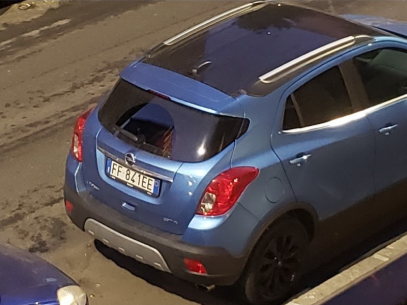
\includegraphics[width=.3\textwidth]{Images/test-photo.png}
            \end{itemize}
            \item The system shows a form to add a license plate and select a type of violation.
            \item Enter the car license plate: FF841EE
            \item Select parking violation.
            \item Press the button to send the report.
            \item The system shows a screen with a “Report sent successfully, thanks for your contribution” message.
        \end{enumerate} \\ \hline
    \textbf{Expected output} & Report submitted, app redirects to home page. \\ \hline
    \textbf{Real output} & Report submitted successfully, confirmed by a notification. App redirects to thank you message. \\ \hline
    \textbf{Outcome} & Partial success, core functionality is working but does not redirect to the home screen as indicated in the RASD. \\ \hline
    \textbf{Alternative flow} & 
        \begin{itemize} \itemsep0em
            \item Backing out of taking a picture after step 2 results in a continuous loading indicator displaying “Taking picture…”.
        \end{itemize} \\ \hline
    
    \end{tabular}
\end{table}

\begin{table}[H]
    \centering
    \begin{tabular}{p{3cm}p{10cm}}
        \textbf{Notes} & The system does not appear to detect license plates in a photo, as the license plate input is always shown.
        Other photos used:
        \begin{center}
            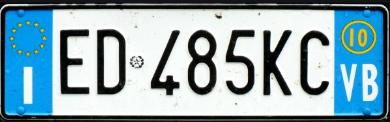
\includegraphics[width=.3\textwidth]{Images/test-photo2.png}
        \end{center}
        \begin{center}
            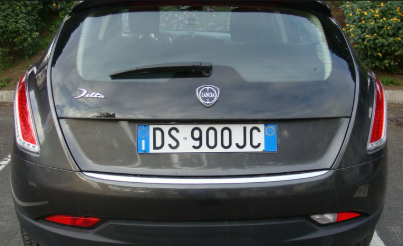
\includegraphics[width=.3\textwidth]{Images/test-photo3.png}
        \end{center}
     \\ \hline
    \end{tabular}
\end{table}

\begin{table}[H]
    \centering
    \begin{tabular}{p{3cm}p{10cm}}
    \textbf{Test ID} & AT-003-REPORT\_HISTORY \\ \hline
    \textbf{Based on} & History report requested by User. \\ \hline
    \textbf{Pre-requisites} & Logged into the app. \\ \hline
    \textbf{Expected steps} & 
        \begin{enumerate} \itemsep0em
            \item Select the report history.
            \item The system shows the report history.
        \end{enumerate} \\ \hline
    \textbf{Real steps} & 
        \begin{enumerate} \itemsep0em
            \item Press the “Get My Report” button.
            \item The system shows the report history.
        \end{enumerate} \\ \hline
    \textbf{Expected output} & The report history is displayed on the screen. \\ \hline
    \textbf{Outcome} & Success \\ \hline
    \end{tabular}
\end{table}

% TODO
\begin{table}[H]
    \centering
    \begin{tabular}{p{3cm}p{10cm}}
    \textbf{Test ID} & AT-004-CHECK\_LICENSE\_PLATE\_VIOLATIONS \\ \hline
    \textbf{Based on} & Checking license plate violations by an Authority. \\ \hline
    \textbf{Pre-requisites} & Logged into the app as an Authority. \\ \hline
    \textbf{Expected steps} & 
        \begin{enumerate} \itemsep0em
            \item Submit multiple reports for a license plate
            \item Go to home screen
            \item Input the license plate code.
            \item The system displays a list of reports for the given license plate ordered by date in descending order.
        \end{enumerate} \\ \hline
    \textbf{Real steps} & 
        \begin{enumerate} \itemsep0em
            \item Submit multiple reports for the license plate: “AS123AS”
            \item Go to home screen
            \item Press “Get License Plate Information”
            \item Input the license plate code “AS123AS”
            \item The system displays a list of reports for the given license plate in no apparent order
        \end{enumerate} \\ \hline
    \textbf{Expected output} & The list of reports for the given license plate is displayed ordered by date in descending order. \\ \hline
    \textbf{Real output} &  The list of reports for the given license plate is displayed in no apparent order. \\ \hline
    \textbf{Outcome} & Partial success, the reports are not sorted as described in the use case. \\ \hline
    \end{tabular}
\end{table}

\begin{table}[H]
    \centering
    \begin{tabular}{p{3cm}p{10cm}}
    \textbf{Test ID} & AT-005-VIOLATION\_NOTIFICATION \\ \hline
    \textbf{Based on} & Real-time notification about nearby violation for an Authority. \\ \hline
    \textbf{Pre-requisites} & Logged into the app as an Authority with the notification service activated. \\ \hline
    \textbf{Expected steps} & 
        \begin{enumerate} \itemsep0em
            \item Submit a report with another phone in close proximity
            \item Receive a notification.
            \item Press the notification message.
            \item The system displays the report, providing the exact location of the report.
        \end{enumerate} \\ \hline
    \textbf{Real steps} & 
        \begin{enumerate} \itemsep0em
            \item Subscribe to notifications for all areas available on the settings screen.
            \item Receive a notification.
            \item System displays a message stating that a new violation was reported in the area.
        \end{enumerate} \\ \hline
    \textbf{Expected output} & The system displays the report with its exact location. \\ \hline
    \textbf{Real output} & The system displays a message indicating the area of the report. \\ \hline
    \textbf{Outcome} & Partial fail, the notifications work but they do not display either the report nor its exact location. \\ \hline
    \textbf{Alternative flow} & 
        \begin{itemize} \itemsep0em
            \item If the app is not open, a system notification pop ups, but when pressed it just opens the app on the screen it was on. If the app was completely closed, it opens it on the home screen.
        \end{itemize} \\ \hline
    \textbf{Note} & One is able to receive notifications while logged in as a normal user, which should not be possible as this functionality is listed as Authority only. \\ \hline
    \end{tabular}
\end{table}


\begin{table}[H]
    \centering
    \begin{tabular}{p{3cm}p{10cm}}
    \textbf{Test ID} & AT-006-LIST\_AREA\_VIOLATIONS \\ \hline
    \textbf{Based on} & List of violations in an area for an Authority. \\ \hline
    \textbf{Pre-requisites} & Logged into the app as an Authority. \\ \hline
    \textbf{Expected steps} & 
        \begin{enumerate} \itemsep0em
            \item Submit multiple reports in a specific area
            \item Go to home screen
            \item Input the area of interest.
            \item The system shows a list of reports in the area.
        \end{enumerate} \\ \hline
    \textbf{Real steps} & 
        \begin{enumerate} \itemsep0em
            \item Submit multiple reports in the same area
            \item Go to home screen
            \item Press “Get Area 1 Violation”
            \item The system shows a list of reports
        \end{enumerate} \\ \hline
    \textbf{Expected output} & The system displays a list of reports inside the given area. \\ \hline
    \textbf{Real output} & The system shows a list of reports, with drastically different coordinates \\ \hline
    \textbf{Outcome} & Fail, the reports shown are in completely different areas. For example one is at (45.6744862, 9.1789748) which is Cabiate, Italy, while another is at (37.4219983, -122.084) which is the Google Campus in California. \\ \hline
    \end{tabular}
\end{table}

\subsection{Other acceptance tests}
Taking into account the functionality implemented, further acceptance tests were performed. However, as there were no use cases for these, there are no expected steps to perform. \\

\begin{table}[H]
    \centering
    \begin{tabular}{p{3cm}p{10cm}}
    \textbf{Test ID} & AT-007-SIGN\_IN \\ \hline
    \textbf{Pre-requisites} & User already signed up to the system. \\ \hline
    \textbf{Real steps} & 
        \begin{enumerate} \itemsep0em
            \item Fill the sign in form with the following data:
            \begin{itemize}[label={}] \itemsep0em
                \item Email: robert@mail.com
                \item Password: robert123
            \end{itemize}
            \item Press the sign in button.
        \end{enumerate} \\ \hline
    \textbf{Expected output} & The system displays the home screen. \\ \hline
    \textbf{Real output} & The system displays the home screen. \\ \hline
    \textbf{Outcome} & Success \\ \hline
    \end{tabular}
\end{table}

\begin{table}[H]
    \centering
    \begin{tabular}{p{3cm}p{10cm}}
    \textbf{Test ID} & AT-009-AREA\_SAFETY \\ \hline
    \textbf{Pre-requisites} & Logged into the application. \\ \hline
    \textbf{Real steps} & 
        \begin{enumerate} \itemsep0em
            \item Press a “Get Area N Safety” button (N could be any of the 3 area numbers).
            \item he system displays a screen indicating a safety estimation and the number of violations reported.
        \end{enumerate} \\ \hline
    \textbf{Expected output} & The system displays the safety of the area. \\ \hline
    \textbf{Real output} & The system displays the safety of the area. \\ \hline
    \textbf{Outcome} & Success \\ \hline
    \end{tabular}
\end{table}


% \begin{table}[H]
%     \centering
%     \begin{tabular}{p{3cm}p{10cm}}
%     \textbf{Test ID} & AT-001-SIGN\_UP \\ \hline
%     \textbf{Based on} & aaaa \\ \hline
%     \textbf{Pre-requisites} & aaaa \\ \hline
%     \textbf{Expected steps} & 
%         \begin{enumerate} \itemsep0em
%             \item aaaaa
%             \item aaaaa
%             \item aaaaa
%             \item aaaaa
%             \item aaaaa
%             \item aaaaa
%         \end{enumerate} \\ \hline
%     \textbf{Real steps} & 
%         \begin{enumerate} \itemsep0em
%             \item aaaaa
%             \item aaaaa
%             \item aaaaa
%             \item aaaaa
%             \item aaaaa
%         \end{enumerate} \\ \hline
%     \textbf{Expected output} &  \\ \hline
%     \textbf{Real output} &  \\ \hline
%     \textbf{Outcome} & Success \\ \hline
%     \textbf{Alternative flow} & 
%         \begin{itemize} \itemsep0em
%             \item aaaaa
%             \item aaaaa
%         \end{itemize} \\ \hline
%     \textbf{Notes} & aaaaa \\ \hline
%     \end{tabular}
% \end{table}
